	\clearpage
\section{Firmware}\label{sec:Firmware}

\todo[inline]{Eine Hardwareplattform. Dongle mit Akku für die BSN und DK für den BMN. Firmware dementsprechend gibt es folgende: BMN, BSN Sensor, BSN Aktor}

\todo[inline]{Räffu: Mesh-5, 7, 8, 9}
\newpage


\subsection{Durchsatz Messung}\label{subsec:DurchsatzMessung}
\todo[inline]{Robin: Mesh-1, 3, 4}

\begin{figure}[H]
	\centering
	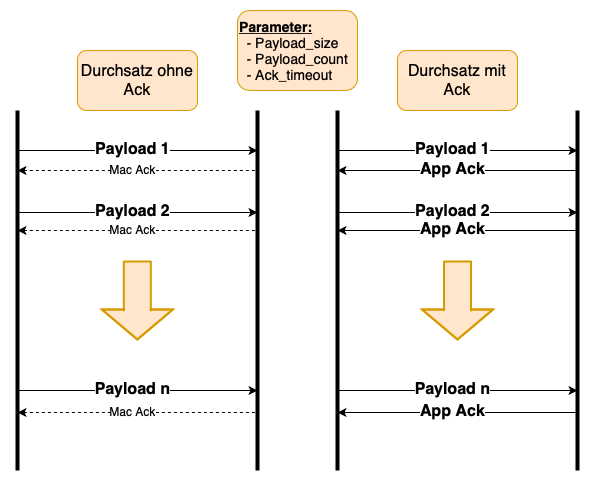
\includegraphics[width=0.5\textwidth]{Durchsatzmessung.png}
	\caption{Konzept Durchsatzmessung}\label{fig:KonzeptDurchsatzmessung}
\end{figure}

\subsection{Latenz Messung}\label{subsec:LatenzMessung}

\begin{figure}[H]
	\centering
	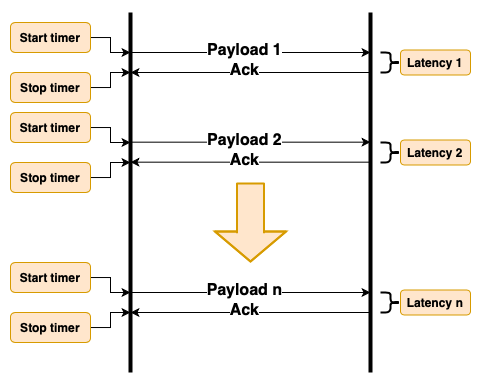
\includegraphics[width=0.5\textwidth]{Latenzmessung.png}
	\caption{Konzept Latenzmessung}\label{fig:Konzept Latenzmessung}
\end{figure}
\newpage



\todo[inline]{Cyrill: Mesh-2, 6, 10}


\subsection{Parameter Mesh Test}\label{subsec:ParameterMeshTest}



